% !TeX spellcheck = en_US

\documentclass{beamer}

\usepackage{amsfonts,amssymb}

\usepackage{tikz}
\usetikzlibrary{shapes,arrows, positioning}

\tikzset{
	treenode/.style = {shape=rectangle, rounded corners,
		draw, align=center, text width=10em,
		fill=red!15},
	root/.style     = {diamond, draw, fill=blue!20, 
		text width=6em, text badly centered, node distance=3cm, inner sep=0pt},
	env/.style      = {treenode, font=\ttfamily\normalsize},
	dummy/.style    = {circle,draw},
	curve/.style={->, thick, >=stealth'},
}
\tikzstyle{line} = [draw, -latex']
\tikzstyle{bag} = [text width=3em, text centered]
\tikzstyle{end} = [rectangle, draw=none, minimum width=2pt, inner sep=0pt]


\mode<presentation> {

% The Beamer class comes with a number of default slide themes
% which change the colors and layouts of slides. Below this is a list
% of all the themes, uncomment each in turn to see what they look like.

%\usetheme{default}
%\usetheme{AnnArbor}
%\usetheme{Antibes}
%\usetheme{Bergen}
%\usetheme{Berkeley}
%\usetheme{Berlin}
%\usetheme{Boadilla}
%\usetheme{CambridgeUS}
%\usetheme{Copenhagen}
%\usetheme{Darmstadt}
%\usetheme{Dresden}
%\usetheme{Frankfurt}
%\usetheme{Goettingen}
%\usetheme{Hannover}
%\usetheme{Ilmenau}
%\usetheme{JuanLesPins}
%\usetheme{Luebeck}
\usetheme{Madrid}
%\usetheme{Malmoe}
%\usetheme{Marburg}
%\usetheme{Montpellier}
%\usetheme{PaloAlto}
%\usetheme{Pittsburgh}
%\usetheme{Rochester}
%\usetheme{Singapore}
%\usetheme{Szeged}
%\usetheme{Warsaw}

% As well as themes, the Beamer class has a number of color themes
% for any slide theme. Uncomment each of these in turn to see how it
% changes the colors of your current slide theme.

%\usecolortheme{albatross}
\usecolortheme{beaver}
%\usecolortheme{beetle}
%\usecolortheme{crane}
%\usecolortheme{dolphin}
%\usecolortheme{dove}
%\usecolortheme{fly}
%\usecolortheme{lily}
%\usecolortheme{orchid}
%\usecolortheme{rose}
%\usecolortheme{seagull}
%\usecolortheme{seahorse}
%\usecolortheme{whale}
%\usecolortheme{wolverine}

%\setbeamertemplate{footline} % To remove the footer line in all slides uncomment this line
\setbeamertemplate{footline}[page number] % To replace the footer line in all slides with a simple slide count uncomment this line

\setbeamertemplate{navigation symbols}{} % To remove the navigation symbols from the bottom of all slides uncomment this line
}

\usepackage{graphicx} % Allows including images
\usepackage{booktabs} % Allows the use of \toprule, \midrule and \bottomrule in tables
%\usepackage {tikz}

\setbeamertemplate{caption}[numbered]

\AtBeginSection[]{
	\begin{frame}
		\vfill
		\centering
		\begin{beamercolorbox}[sep=8pt,center,shadow=true,rounded=true]{title}
			\usebeamerfont{title}\insertsectionhead\par%
		\end{beamercolorbox}
		\vfill
	\end{frame}
}

%\usepackage {xcolor}
\definecolor {processblue}{cmyk}{0.96,0,0,0}
%----------------------------------------------------------------------------------------
%	TITLE PAGE
%----------------------------------------------------------------------------------------

\title[Short title]{Learning (not) to trade} % The short title appears at the bottom of every slide, the full title is only on the title page

\author{Teodor Godina \and Serge Kassibrakis \and Semyon Malamud 
	\\ 
	Alberto Teguia \and Jiahua (Java) Xu} % Your name
\institute[EPFL]
{
Swissquote, EPFL, SFI, UBC \\ % Your institution for the title page
\medskip
}
\date{\today} % Date, can be changed to a custom date

\begin{document}

\begin{frame}
\titlepage % Print the title page as the first slide
\end{frame}

%\begin{frame}
%\frametitle{Overview} % Table of contents slide, comment this block out to remove it
%\tableofcontents % Throughout your presentation, if you choose to use \section{} and \subsection{} commands, these will automatically be printed on this slide as an overview of your presentation
%\end{frame}

%----------------------------------------------
%	PRESENTATION SLIDES
%----------------------------------------------

\section{Two quick surveys}

\begin{frame}[allowframebreaks]{Survey}
	\begin{block}{}
		Imagine you are a stock trader. You have performed very \textcolor{blue}{well} during the last year:
		\textcolor{blue}{$10\%$} of return. Now you wonder whether to keep trading or exit.
	\end{block}

Other things equal, you'd be more likely to exit, if you:

\begin{enumerate}[A]
	\item have been trading for 10 years
	\item have been trading for 2 years
\end{enumerate}

\includegraphics[scale=0.1]{figures/happymoney}

\framebreak

	\begin{block}{}
		Imagine you are a stock trader. You have performed very \textcolor{red}{poorly} during the last year:
		\textcolor{red}{$-10\%$} of return. Now you wonder whether to keep trading or exit.
	\end{block}
	
	Other things equal, you'd be more likely to exit, if you:
	
	\begin{enumerate}[A]
		\item have been trading for 10 years
		\item have been trading for 2 years
	\end{enumerate}
	
	\includegraphics[scale=0.2]{figures/sadmoney}
	
\end{frame}


\section{Research motivation and background}

\begin{frame}{Exit procrastination?}
	
	\begin{figure}
	\includegraphics[width=0.85\linewidth,trim={10 30 0 0},clip]{figures/pltexitgivenT-1}
	\caption{Given calendar time (2014-12-31) and trading performance (return), empirical exit likelihood decreases with age}
	\end{figure}

\end{frame}


\begin{frame}{Why is it relevant?}
	
	\begin{enumerate}
		\item{Trading platforms}
		\begin{itemize}
			\item should focus on retaining inexperienced traders
		\end{itemize}

		\item{Investors}
		\begin{itemize}
			\item should understand their trading inertia might not be economically rational
		\end{itemize}
	\end{enumerate}
	

\end{frame}


\begin{frame}{Literature review}
	
	\begin{itemize}
		\item \cite{Seru2010}: two learning routes of investors---the first type improves over time by learning from their trading experience, while the second type realizes their ability is insufficient and ceases to trade.
		\item \cite{Nicolosi2009}: investors benefit from trading experience and can learn to place more profitable trades.
		\item \cite{Gervais2001}: traders develop assessments of their own trading ability through experience.
		\item \cite{Schraeder2015}: young investors trade frequently but obtain lower returns.
		
		%		Also relevant for our study is the literature on the trading behavior of different investor cohorts.  \cite{Grinblatt2001} show that domestic and less sophisticated investors tend to be reversal traders, whereas foreign and more sophisticated investors tend to be trend followers. \cite{Dorn2005} investigate the relationship between investor behaviors and objective attributes such age, gender and income, as well as subjective attributes such as self-reported risk attitude. They find that investors with high risk tolerance and who believe themselves to be more knowledgeable than the average trade more aggressively. \cite{Kourtidis2011} find that wealthy and educated individuals are associated with higher risk tolerance and more frequent trading.
		%		
		%		Our research is also informed by the vast literature on investor psychology. Many such research studies focus on investor overconfidence demonstrated by excessive and/or aggressive trading. \cite{Odean1998} proves that overconfidence in one's information increases one's trading volume, and that overconfidence when manifested by miscalibration, decreases the expected utility of overconfident traders. \cite{Odean1999} demonstrates that investors with reduced trading costs tend to trade excessively, resulting in unsuccessful investments. \cite{Glaser2007} find that investors' overconfidence, when measured by better-than-average effect, is positively related to trading volume; overconfidence measured by miscalibration, however, has little to do with trading volume. \cite{Barber2000} conclude that individuals who trade excessively often gain lower net returns as the superior trading performance does not always compensate for the higher trading costs. \cite{Daniel2015} suggest that unprofitable but excessive active trading can be explained by overconfident beliefs in one's own talents and abilities.
		%		
		%		Other research studies discuss the disposition effect --  to sell winners and ride losers – a theory established by  \cite{Shefrin1985}. \cite{Odean1998a} demonstrates investors preference for realizing winners over losers, except in the tax optimizing period of December. \cite{Dhar2006} suggest educated individuals exhibit lower disposition bias than their less literate peers. Relatedly, \cite{Kahneman1979} suggest people unwilling to accept losses tend to engage in gambles that are riskier than they would normally tolerate.
		
	\end{itemize}
	
\end{frame}


\section{Methodology}

\begin{frame}{Data}
	
\begin{itemize}
	\item Source: one of the biggest stock trading platforms for retail traders in Switzerland
	\item $82,072$ traders' status (exit/remain) from 2001-05-04 to 2019-01-29
	\item $90,628$ traders' trading activity (buy/sell) from 2001-05-08 to 2018-12-31,
	with in total $6,766,393$ trader-action observations
	\item $64,037$ traders' daily account value from 2009-01-01 to 2018-12-28, 
	with in total $107,332,300$ account-day observations
\end{itemize}
	
\end{frame}


\begin{frame}[allowframebreaks]{The model}
\framesubtitle{Assumptions}

\begin{itemize}
	
	\item Based on their trading skills, each trader falls in either of the two categories: (i) with trading skills, i.e. good type, denoted by $G$, or (ii) without trading skills, i.e. bad type, denoted by $B$. 
	
	\item Traders do not know their types, but have a prior belief about their probability of being Type $G$ equal to $\pi_0$.
	
	\item Type $B$ traders never place successful trades with profits sufficient to cover the total trading cost.
	
	\item For type $G$ traders, successful trades arrive at jump times of a time-inhomogeneous Poisson process, $N_t$, with an exogenously given intensity $f(t)$, namely, $\mathbb P[N_{t+dt}-N_t = 1] = f(t)dt$.
	
	\item Type $G$ traders improve their trading skills with experience. Thus, $f(t)$ is a monotone increasing function of the trader's trade age, $t$.
	
	\item Traders learn about their types and continuously update their belief $\pi_t$ from observing their trading history.
	
	\item Entry of new traders happens at a constant rate $\rho_{entry}$. 
	
	\item Traders exit from trading for two reasons: (i) an exogenous ``exit shock" that occurs at a Poisson intensity $\rho_{exit}$, or (ii) the trader's posterior probability of being Type $G$ dropping below a threshold value, i.e. when the trader becomes sufficiently confident that he is Type $B$.
	
	\item Each trader's trading cost follows a quadratic function $C(\varphi, \eta) =\varphi + 0.5 c^{-1} \eta^2$ for some small $c>0$, where  $\varphi$ represents a trader's idiosyncratic running fixed cost of trading, and $\eta$ represents a trader's trading effort that increases the probability of success by $e$ from some minimal level.
\end{itemize}
\end{frame}


\begin{frame}[allowframebreaks]{Time-inhomogeneous Poisson process}
The arrival of success becomes increasingly frequent for Type $G$.

	\begin{columns}[t]
		\begin{column}{0.49\textwidth}
			\begin{block}{$f(t)=-10e^{-0.02t}+20$}
				\begin{figure}
					\includegraphics[width=\linewidth]{figures/funcf2}
				\end{figure}
			\end{block}  
		\end{column}
	
	\begin{column}{0.49\textwidth}
					\begin{block}{$f(t)=-1.5e^{-0.02t}+2$}
			\begin{figure}
				\includegraphics[width=\linewidth]{figures/funcf1}
			\end{figure}
		\end{block}  
	\end{column}
\end{columns}

\framebreak

Cum. prob. of no. of successes $n$ achieved by age $t$
(\textcolor{green}{green}-\textcolor{orange}{orange} fan):
$\mathbb{P}[N_t < n]
=  \sum_{k=0}^{n-1} \frac{\left(F(t)\right)^k}{e^{F(t)}k!}$

Expected no. of successes $n$ by age $t$ for Type $G$
(\textcolor{red}{red}
line):
$\mathbb{E}[N_{t}] = F(t)=\int_0^t f(t) dt$

	\begin{columns}[t]
		\begin{column}{0.49\textwidth}
			\begin{block}{$f(t)=-10e^{-0.02t}+20$}
				\begin{figure}
					\includegraphics[width=\linewidth]{figures/probn2}
				\end{figure}
			\end{block}  
		\end{column}
		
		\begin{column}{0.49\textwidth}
			\begin{block}{$f(t)=-1.5e^{-0.02t}+2$}
				\begin{figure}
					\includegraphics[width=\linewidth]{figures/probn1}
				\end{figure}
			\end{block}  
		\end{column}
	\end{columns}

\framebreak

Probability of experiencing $n$ successes by age $t$ for Type $G$
(\textcolor{blue}{c}\textcolor{orange}{o}\textcolor{green}{l}\textcolor{red}{o}\textcolor{violet}{r} lines):
$
\mathbb{P}[\tau \leq t \,|\, N_{\tau} = n]
= 1 - \sum_{k=0}^{n-1} \frac{\left(F(t)\right)^k}{e^{F(t)}k!}
$

Expected time needed to achieve $n$ successes (black diamonds):
$
\mathbb{E}[t \,|\, N_t = n] = \int_0^{\infty} \frac{tf(t)(F(t))^{n-1}}{e^{F(t)}(n - 1)!} dt
$
	\begin{columns}[t]
		\begin{column}{0.49\textwidth}
			\begin{block}{$f(t)=-10e^{-0.02t}+20$}
				\begin{figure}
					\includegraphics[width=\linewidth]{figures/cdft2}
				\end{figure}
			\end{block}  
		\end{column}
		
		\begin{column}{0.49\textwidth}
			\begin{block}{$f(t)=-1.5e^{-0.02t}+2$}
				\begin{figure}
					\includegraphics[width=\linewidth]{figures/cdft1}
				\end{figure}
			\end{block}  
		\end{column}
	\end{columns}


\framebreak

The belief of being Type $G$ decreases before encountering the first success.

$\pi(t) = \frac{1}{(\frac{1}{\pi_0}-1) e^{F(t)}+1},\ t<\tau_N$

\begin{columns}[t]
	\begin{column}{0.49\textwidth}
		\begin{block}{$f(t)=-10e^{-0.02t}+20$}
			\begin{figure}
				\includegraphics[width=\linewidth]{figures/pis2}
			\end{figure}
		\end{block}  
	\end{column}
	
	\begin{column}{0.49\textwidth}
		\begin{block}{$f(t)=-1.5e^{-0.02t}+2$}
			\begin{figure}
				\includegraphics[width=\linewidth]{figures/pis1}
			\end{figure}
		\end{block}  
	\end{column}
\end{columns}

\end{frame}



\begin{frame}[allowframebreaks]{Evolution of belief}
\begin{block}{}
	
	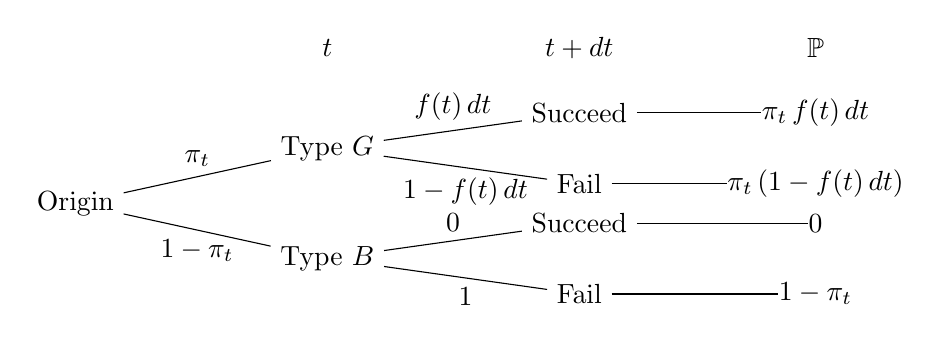
\begin{tikzpicture}[
level distance=3.2cm,
level 1/.style={sibling distance=1.4cm},
level 2/.style={sibling distance=0.9cm},
level 3/.style={level distance =3cm},
grow'=right]
\tikzstyle{every node}=[]
\node (Root) [] {Origin}
child [] {
	node {Type $G$}
	child { node {Succeed} 
		child {node[end] {$\pi_t \, f(t)\,dt$} }
		edge from parent
		node[above] {$f(t)\,dt$}
	}
	child [black] { node {Fail} 
		child {node[end] {$\pi_t \, (1 - f(t)\,dt)$} }
		edge from parent
		node[below] {$1-f(t)\,dt$}
	}
	edge from parent
	node[above] {$\pi_t$}
}
child {
	node {Type $B$}
	child { node {Succeed} 
		child {node[end] {$0$} }
		edge from parent
		node[above] {$0$}
	}
	child { node {Fail} 
		child {node[end] {$1-\pi_t$} }
		edge from parent
		node[below] {$1$}
	}
	edge from parent
	node[below] {$1-\pi_t$}
}
;
% How I'm applying labels to each level. 
% Need to be able to dynamically align nodes at top level
\begin{scope}[every node/.style={align=center, anchor=center, font=\bfseries,}]
\node[above= 0.4cm of Root-1-1-1] (labels-level) {$\mathbb{P}$};
\node[at =(labels-level-|Root-1-1)] {$t+dt$};
\node[at =(labels-level-|Root-1)] {$t$};

\end{scope}
\end{tikzpicture}

\end{block}

$$
d\pi_t = 
\pi_{t+dt} - \pi_t  = \frac{\pi_t\big(1-f(t)dt\big)}{\pi\big(1-f(t)dt\big)+(1-\pi_t)}  - \pi_t
 = -f(t)\pi_t (1-\pi_t)dt
$$
for $t<\tau_N,$ while $\pi_t=1$ for $t\ge \tau_N.$ 

\framebreak

Log transformation for mathematical convenience:
$$
\ell_t\ =\ \ln\frac{\pi_t}{1-\pi_t}
$$

By direct calculation, $\ell_t$ follows the dynamics:
$$
d\ell_t\ =\ -f(t)dt
$$ for $t<\tau_N$ and $\ell_t=\infty$ for $t\ge \tau_N.$
\end{frame}


\begin{frame}
\begin{figure}[h!]
	\centering
	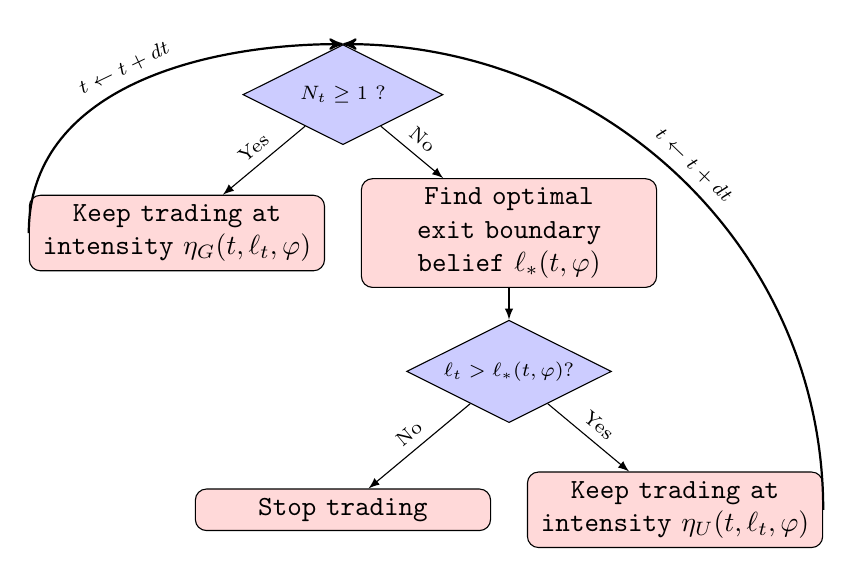
\begin{tikzpicture}
	[
	grow                    = down,
	sibling distance        = 12em,
	level distance          = 5em,
	edge from parent/.style = {draw, -latex},
	every node/.style       = {font=\scriptsize},
	sloped
	]
	\node[root, aspect=2](count){
		$ N_t \ge 1$ ?
	}
	child{node[env](keepg){
			Keep trading at intensity $\eta_G(t, \ell_t, \varphi)$
		}
		edge from parent node [above]{
			Yes
	}}
	child{node[env]{
			Find optimal exit boundary belief $\ell_*(t, \varphi)$
		}
		child{node[root, aspect=2](compare){
				$\ell_t > \ell_*(t, \varphi)$?
			}
			child {node[env]{
					Stop trading
				}
				edge from parent node [above]{
					No
			}}
			child {node[env](keepb){
					Keep trading at intensity $\eta_U(t, \ell_t, \varphi)$
				}
				edge from parent node [above]{
					Yes
			}}
			edge from parent node [below]{}}
		edge from parent node [above]{No} };
	
	\draw [curve] (keepb.east) to[out=90, in=0] node[above,midway]{$t \leftarrow t + dt$} (count.north);
	\draw [curve] (keepg.west) to[out=90, in=180] node[above,midway]{$t \leftarrow t + dt$} (count.north);
	\end{tikzpicture}
	\caption{A trader's decision tree involving effort cost (absent exogenous shock)}
	\label{fig:decision2}
\end{figure}
\end{frame}


\begin{frame}
	
\begin{block}{Value functions}
	\begin{itemize}
		\item 	Type $G$:
		
		$
		V_G(t, \varphi)\ =\ \int_t^\infty e^{-r(s-t)}\big(f(s)-(\varphi + 0.5 c^{-1} \eta^2)\big)ds\
		$
		
		\item Type unknown:
		
		$
		V(\ell, t, \varphi)\ =\ \max_{\tau_E} \mathbb{E}\Big[
		-\int_t^{\min\{\tau_E,\tau_N\}}  e^{-r s} (\varphi + 0.5 c^{-1} \eta^2) ds\ +\ e^{-r\tau_N} {\bf 1}_{\tau_N<\tau_E}\big(1\ +\ V_G(\tau_N,\varphi)\big)\Big]
		$
	\end{itemize}
\end{block}

\begin{block}{Theorems}
		\begin{itemize}
		\item exit boundary $\ell_*(t,\varphi)$
		
			$\frac{e^{\ell_*(t,\varphi)}}{e^{\ell_*(t,\varphi)}+1}\ =\ \frac{\varphi}{f(t)(1+V_G(t,\varphi))} $
		\item 	Trading intensity Type $G$:
		
		$
\eta_G\ =\ c f(t)
		$
		
		\item Trading intensity Type unknown:
		
$\eta_U\ =\ c\Big(-V_\ell (\ell, t;c) f(t)\ +\ \pi(\ell) f(t) \big(1+V_G(t;c) - V(\ell, t;c)\big)\Big)$
	\end{itemize}

\end{block}

\end{frame}

\begin{frame}[allowframebreaks]{Variables and parameters}
	\begin{block}{Observable}
		\begin{itemize}
			\item $1_{exit}$: account status---closed/open
			\item $\eta$ individual trading intensity: one-year trading volume (CHF) or count (times)
			\item $R$ individual trading performance: one-year excess log return
			\item $t$ trading age: time since account open
			\item $\bar M(t)$ total trading mass by age: number of open accounts
		\end{itemize}
	\end{block}
	
	\begin{block}{Unobservable}
		\begin{itemize}
			\item Success
			\item Type ($G$ or $B$) and its distribution
			\item $\ell$ belief of being Type $G$ and its (conditional) distribution (given type)
			\item $\varphi$ running cost and its distribution
			\item Conditional distribution (given type and belief) of $R$
			\item $\rho_{exit}$ exit rate due to exogenous shock
		\end{itemize}
	\end{block}
	
	\framebreak
	
	\begin{block}{Other}
		\begin{itemize}
			\item $c$ cost factor per trading effort: arbitrarily fixed
			\item $\rho_{entry}$ entry rate: assumed time invariant
		\end{itemize}
		
		\includegraphics[
		width = 0.7\textwidth]{figures/rouentry-1}
	
	\end{block}
\end{frame}


\begin{frame}[allowframebreaks]{Trading mass}
	
\begin{columns}
	\begin{column}{0.49\textwidth}
		\begin{block}{Empirical, entry rate unnormalized}
			\begin{figure}
					\includegraphics[
					height=0.38\textheight,trim={0 30 35 15},clip
					]{figures/rouentry-2}
			\end{figure}
		\end{block}  
	\end{column}
	
	\begin{column}{0.49\textwidth}
		\begin{block}{Model}
			\begin{figure}
				\includegraphics[height=0.385\textheight]{figures/MassThruTime}
			\end{figure}
		\end{block}  
	\end{column}
\end{columns}

\framebreak
	
	\begin{columns}
		\begin{column}{0.49\textwidth}
			\begin{block}{Empirical, entry rate normalized}
				\begin{figure}
					\includegraphics[
					height=0.38\textheight,trim={0 30 35 15},clip
					]{figures/rouentry-3}
				\end{figure}
			\end{block}  
		\end{column}
		
		\begin{column}{0.49\textwidth}
			\begin{block}{Model}
				\begin{figure}
					\includegraphics[height=0.385\textheight]{figures/MassThruTime}
				\end{figure}
			\end{block}  
		\end{column}
	\end{columns}

\framebreak

\begin{columns}
	\begin{column}{0.49\textwidth}
		\begin{block}{Empirical, entry rate unnormalized}
			\begin{figure}
				\includegraphics[
				height=0.38\textheight,trim={0 30 35 15},clip
				]{figures/massdist-1}
			\end{figure}
		\end{block}  
	\end{column}
	
	\begin{column}{0.49\textwidth}
		\begin{block}{Model}
			\begin{figure}
				\includegraphics[height=0.385\textheight]{figures/totalmass}
			\end{figure}
		\end{block}  
	\end{column}
\end{columns}

\framebreak

\begin{columns}
	\begin{column}{0.49\textwidth}
		\begin{block}{Empirical, entry rate normalized}
			\begin{figure}
				\includegraphics[
				height=0.38\textheight,trim={0 30 35 15},clip
				]{figures/massdist-2}
			\end{figure}
		\end{block}  
	\end{column}
	
	\begin{column}{0.49\textwidth}
		\begin{block}{Model}
			\begin{figure}
				\includegraphics[height=0.385\textheight]{figures/totalmass}
			\end{figure}
		\end{block}  
	\end{column}
\end{columns}

\end{frame}


\begin{frame}[allowframebreaks]{Further assumptions}
	\begin{itemize}
\item Success arrival intensity: $f(t)=\alpha \, e^\beta + \gamma$, where $\alpha = -10, \beta = -0.02, \gamma = 20$
\item Discount rate: $r = 0.1$
\item Constant entry rate: $\rho_{entry} = 1$
\item Exit rate due to exogenous shock: $\rho_{exit} = 0.4$
\item $c$ cost factor: 0.05
\end{itemize}

\framebreak

\begin{itemize}
\item Distribution of types at entry: Type $G$ 10\%, Type $B$ 90\%
\item Distribution of $\varphi$ at entry: uniform distribution on $[0, \varphi^*]$, where $\varphi^* = \alpha + \gamma - 0.5 \, (r + \frac{\alpha \, \beta}{\alpha + \gamma})$
\item Distribution of belief $\ell_0$ at entry: inverse exponential distribution with $\lambda = 60$ for Type $G$ and $\lambda = 50$ for Type $B$, on $[\ell(0, \varphi), +\infty)$
\item Distribution of return based on true type and belief:
\begin{itemize}
	\item Being $G$ believing $G$: $\mathbb N(2, 0.8^2)$
	\item Being $G$ believing $B$: $\mathbb N(1, 1^2)$
	$\leftarrow$ \textit{underconfidence}
	\item Being $B$ believing $G$: $\mathbb N(-2, 1^2)$
	$\leftarrow$ \textit{overconfidence}
	\item Being $B$ believing $B$: $\mathbb N(-1, 1.2^2)$
\end{itemize}
	\end{itemize}
\end{frame}



\section{Empirical and modeling results}

\begin{frame}{Belief lower boundary $\ell_*(t, \varphi)$}
	\begin{figure}
	\colorbox{white}{
		\includegraphics[
		height=0.7\textheight
		]{figures/lstar}}
	\end{figure}

$\ell_*(t, \varphi)$ decreases with $t$---but does that translate into exit procrastination?
\end{frame}



\begin{frame}[allowframebreaks]{Trading intensity}
	
	Trading intensity: all traders that have stayed up to 5 years
	
	\begin{columns}[t]
		\begin{column}{0.49\textwidth}
			\begin{block}{Empirical: trading volume (CHF)}
				\begin{figure}
						\includegraphics[
						height=0.38\textheight,trim={0 30 0 15},clip
						]{figures/trintfolonecohort-1}
				\end{figure}
			\end{block}  
		\end{column}
		
		\begin{column}{0.49\textwidth}
			\begin{block}{Empirical: trading count}
				\begin{figure}
						\includegraphics[
						height=0.38\textheight,trim={0 30 0 15},clip
						]{figures/trintfolonecohort-4}
				\end{figure}
			\end{block}  
		\end{column}
	\end{columns}
	
	\framebreak
	
		Trading intensity: all traders that have stayed up to 10 years
	
	\begin{columns}[t]
		\begin{column}{0.49\textwidth}
			\begin{block}{Empirical: trading volume (CHF)}
				\begin{figure}
						\includegraphics[
						height=0.38\textheight,trim={0 30 0 15},clip
						]{figures/trintfolonecohort-2}
				\end{figure}
			\end{block}  
		\end{column}
		
		\begin{column}{0.49\textwidth}
			\begin{block}{Empirical: trading count}
				\begin{figure}
						\includegraphics[
						height=0.38\textheight,trim={0 30 0 15},clip
						]{figures/trintfolonecohort-5}
				\end{figure}
			\end{block}  
		\end{column}
	\end{columns}
	
	\framebreak
	
		Trading intensity: all traders that have stayed up to 15 years
	
	\begin{columns}[t]
		\begin{column}{0.49\textwidth}
			\begin{block}{Empirical: trading volume (CHF)}
				\begin{figure}
						\includegraphics[
						height=0.38\textheight,trim={0 30 0 15},clip
						]{figures/trintfolonecohort-3}
				\end{figure}
			\end{block}  
		\end{column}
		
		\begin{column}{0.49\textwidth}
			\begin{block}{Empirical: trading count}
				\begin{figure}
						\includegraphics[
						height=0.38\textheight,trim={0 30 0 15},clip
						]{figures/trintfolonecohort-6}
				\end{figure}
			\end{block}  
		\end{column}
	\end{columns}
	
	\framebreak
	
	Trading intensity---trading age curve: convex
	
	Intuition: two opposing forces that influence trading intensity
	
	\begin{enumerate}
		\item positive: learning experience increases success likelihood for Type $G$
		\item negative: belief of being type $G$ decreases before 1st success
	\end{enumerate}
	
	\begin{columns}[t]
		\begin{column}{0.49\textwidth}
			\begin{block}{Empirical: trading volume (CHF)}
				\begin{figure}
					\colorbox{white}{
						\includegraphics[
						height=0.38\textheight,trim={0 30 35 15},clip
						]{figures/pltexit-5}}
				\end{figure}
			\end{block}  
		\end{column}
		
		\begin{column}{0.49\textwidth}
			\begin{block}{Empirical: trading count}
				\begin{figure}
					\colorbox{white}{
						\includegraphics[
						height=0.38\textheight,trim={0 30 35 15},clip
						]{figures/pltexit-6}}
				\end{figure}
			\end{block}  
		\end{column}
	\end{columns}

\framebreak

$
\eta_B(\ell, \varphi, t)\ =\ c\Big(-V_\ell (\ell, t, \varphi) f(t)\ +\ \pi(\ell) f(t) \big(1+V_G(t, \varphi) - V(\ell, t, \varphi)\big)\Big)
$

$
\eta_G(\varphi, t)\ =\ c f(t)
$
	\begin{columns}[t]
	\begin{column}{0.49\textwidth}
		\begin{block}{Empirical}
			\begin{figure}
				\colorbox{white}{
					\includegraphics[
					height=0.38\textheight,trim={0 30 35 15},clip
					]{figures/pltexit-7}}
			\end{figure}
		\end{block}  
	\end{column}
	
	\begin{column}{0.49\textwidth}
		\begin{block}{Empirical: initial belief $\ell_0=9$}
			\begin{figure}
				\includegraphics[height=0.407\textheight]{figures/trintgivenlphi9}
			\end{figure}
		\end{block}  
	\end{column}
\end{columns}

\framebreak

$
\eta_B(\ell, \varphi, t)\ =\ c\Big(-V_\ell (\ell, t, \varphi) f(t)\ +\ \pi(\ell) f(t) \big(1+V_G(t, \varphi) - V(\ell, t, \varphi)\big)\Big)
$

$
\eta_G(\varphi, t)\ =\ c f(t)
$

\begin{columns}[t]
	\begin{column}{0.49\textwidth}
		\begin{block}{Empirical}
			\begin{figure}
				\colorbox{white}{
					\includegraphics[
					height=0.38\textheight,trim={0 30 35 15},clip
					]{figures/pltexit-7}}
			\end{figure}
		\end{block}  
	\end{column}
	
	\begin{column}{0.49\textwidth}
		\begin{block}{Empirical: initial belief $\ell_0=12$}
			\begin{figure}
				\includegraphics[height=0.407\textheight]{figures/trintgivenlphi12}
			\end{figure}
		\end{block}  
	\end{column}
\end{columns}

\framebreak

$
\eta_B(\ell, \varphi, t)\ =\ c\Big(-V_\ell (\ell, t, \varphi) f(t)\ +\ \pi(\ell) f(t) \big(1+V_G(t, \varphi) - V(\ell, t, \varphi)\big)\Big)
$

$
\eta_G(\varphi, t)\ =\ c f(t)
$


\begin{columns}[t]
	\begin{column}{0.49\textwidth}
		\begin{block}{Empirical}
			\begin{figure}
				\colorbox{white}{
					\includegraphics[
					height=0.38\textheight,trim={0 30 35 15},clip
					]{figures/pltexit-7}}
			\end{figure}
		\end{block}  
	\end{column}
	
	\begin{column}{0.49\textwidth}
		\begin{block}{Empirical: initial belief $\ell_0=15$}
			\begin{figure}
				\includegraphics[height=0.407\textheight]{figures/trintgivenlphi15}
			\end{figure}
		\end{block}  
	\end{column}
\end{columns}
\end{frame}



\begin{frame}{Initial belief distribution}
	Inverse exponential distribution on 
	$[\ell - \ell_*(0, \varphi), +\infty)$
	
	\begin{columns}[t]
	\begin{column}{0.49\textwidth}
		\begin{block}{$\varphi = 0.01$}
			\begin{figure}
				\includegraphics[width=\linewidth]{figures/ldist1}
			\end{figure}
		\end{block}  
	\end{column}
	
	\begin{column}{0.49\textwidth}
		\begin{block}{$\varphi = 9$}
			\begin{figure}
				\includegraphics[width=\linewidth]{figures/ldist2}
			\end{figure}
		\end{block}  
	\end{column}
\end{columns}
\end{frame}


\begin{frame}{Average trading intensity}


	
	\begin{columns}[t]
		\begin{column}{0.49\textwidth}
		\begin{block}{Empirical}
	\begin{figure}
		\colorbox{white}{
			\includegraphics[
			height=0.38\textheight,trim={0 30 35 15},clip
			]{figures/pltexit-7}}
	\end{figure}
\end{block}  
\end{column}
		
		\begin{column}{0.49\textwidth}
			\begin{block}{Model}
				\begin{figure}
					\includegraphics[height=0.41\textheight]{figures/intensity}
				\end{figure}
			\end{block}  
		\end{column}
	\end{columns}
\end{frame}



\begin{frame}[allowframebreaks]{Average return}
	
		\begin{columns}[t]
		\begin{column}{0.49\textwidth}
			\begin{block}{Empirical}
				\begin{figure}
					\colorbox{white}{
						\includegraphics[
						height=0.38\textheight,trim={0 30 35 10},clip
						]{figures/rtn-1}}
				\end{figure}
			\end{block}  
		\end{column}
		
		\begin{column}{0.49\textwidth}
			\begin{block}{Model}
				\begin{figure}
					\includegraphics[height=0.41\textheight]{figures/avgreturn}
				\end{figure}
			\end{block}  
		\end{column}
	\end{columns}


\framebreak

	\begin{columns}[t]
		\begin{column}{0.49\textwidth}
			\begin{block}{Empirical}
				\begin{figure}
					\colorbox{white}{
						\includegraphics[
						height=0.38\textheight,trim={0 30 35 10},clip
						]{figures/rtn-2}}
				\end{figure}
			\end{block}  
		\end{column}
		
		\begin{column}{0.49\textwidth}
			\begin{block}{Model}
				\begin{figure}
					\includegraphics[height=0.41\textheight]{figures/avgreturn}
				\end{figure}
			\end{block}  
		\end{column}
	\end{columns}
\end{frame}


\begin{frame}[allowframebreaks]{Exit}
	
At a given calendar time and return level, exit likelihood decreases with trading age.
	
	\begin{columns}[t]
		\begin{column}{0.49\textwidth}
			\begin{block}{Empirical}
				\begin{figure}
					\colorbox{white}{
						\includegraphics[
						height=0.38\textheight,trim={20 30 35 40},clip
						]{figures/pltexitgivenT-1}}
				\end{figure}
			\end{block}  
		\end{column}
		
		\begin{column}{0.49\textwidth}
			\begin{block}{Model}
				\begin{figure}
					\includegraphics[height=0.412\textheight]{figures/exitgivenRT2}
				\end{figure}
			\end{block}  
		\end{column}
	\end{columns}


\framebreak


At a given calendar time and return level, exit likelihood decreases with trading age.


	\begin{columns}[t]
	\begin{column}{0.49\textwidth}
		\begin{block}{Empirical: 2014-12-31}
			\begin{figure}
				\colorbox{white}{
					\includegraphics[
					height=0.38\textheight,trim={20 30 35 15},clip
					]{figures/pltexit-2}}
			\end{figure}
		\end{block}  
	\end{column}
	
	\begin{column}{0.49\textwidth}
		\begin{block}{Model}
			\begin{figure}
				\includegraphics[height=0.412\textheight]{figures/ExitLikeliR}
			\end{figure}
		\end{block}  
	\end{column}
\end{columns}


\framebreak


At a given calendar time and return level, exit likelihood decreases with trading age.


\begin{columns}[t]
	\begin{column}{0.49\textwidth}
		\begin{block}{Empirical: 2016-12-31}
			\begin{figure}
				\colorbox{white}{
					\includegraphics[
					height=0.38\textheight,trim={20 30 35 15},clip
					]{figures/pltexit-3}}
			\end{figure}
		\end{block}  
	\end{column}
	
	\begin{column}{0.49\textwidth}
		\begin{block}{Model}
			\begin{figure}
				\includegraphics[height=0.412\textheight]{figures/ExitLikeliR}
			\end{figure}
		\end{block}  
	\end{column}
\end{columns}
\end{frame}

\begin{frame}{Summary}
We build a model which demonstrates, in accordance with empirical findings, that:
\begin{itemize}
\item Experienced traders perform on average better than inexperienced traders.
\item Nevertheless, survivorship bias does not explain everything: at a given performance level, experienced traders are less likely to exit than inexperienced traders.
\begin{itemize}
	\item There exists a downward moving exit boundary.
\end{itemize}
\item Inexperienced traders trade more intensively, possibly in order to discover their trading skill level.
\end{itemize}
\end{frame}


\begin{frame}[allowframebreaks]{References}
	\bibliographystyle{apalike}
	\bibliography{trading}
\end{frame}


\begin{frame}
\Huge{\centerline{The End}}
\end{frame}

\end{document}
